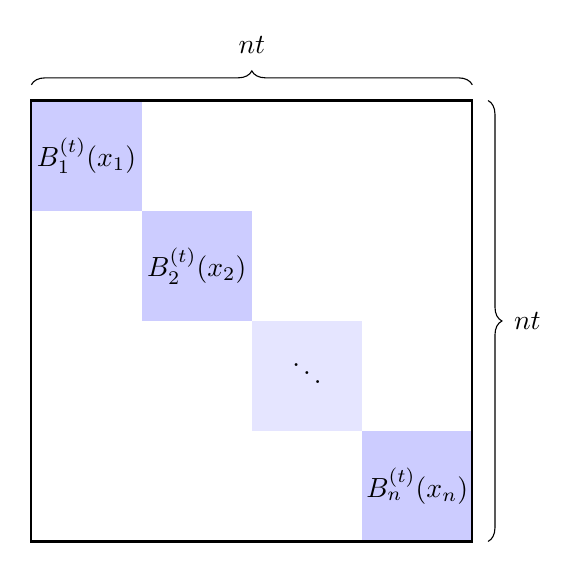
\begin{tikzpicture}[scale = 1.4]
		
	\fill[blue!20] (0,4) rectangle (1,3);
	\fill[blue!20] (1,3) rectangle (2,2);
	\fill[blue!10] (2,2) rectangle (3,1);
	\fill[blue!20] (3,1) rectangle (4,0);
	
	\draw[thick] (0,0) rectangle (4,4);
	
	\node at (0.5, 3.5) {$B^{(t)}_1(x_1)$};
	\node at (1.5, 2.5) {$B^{(t)}_2(x_2)$};
	\node at (2.5, 1.6) {$\ddots$};
	\node at (3.5, 0.5) {$B^{(t)}_n(x_n)$};
	
	% \node at (-0.8, 2) {$B^{(t)}(x)\ =$};
	
	\draw [decorate,decoration={brace, amplitude=5pt, raise=2mm}]
	(0,4) -- (4,4) node[midway, yshift=7mm]{$nt$};
	
	\draw [decorate,decoration={brace, amplitude=5pt, raise=2mm}]
	(4,4) -- (4,0) node[midway, xshift=7mm]{$nt$};
	
\end{tikzpicture}
